\documentclass[12pt,twocolumn,letterpaper]{article}

%% Language and font encodings
\usepackage[english]{babel}
\usepackage[utf8x]{inputenc}
\usepackage[T1]{fontenc}

%% margins
\usepackage[margin=0.8in]{geometry}

%% captions
\usepackage[width=.45\textwidth]{caption}

%% Sets page size and margins
%\usepackage[a4paper,top=3cm,bottom=2cm,left=3cm,right=3cm,marginparwidth=1.75cm]{geometry}

% make title page/contents one column (use the begin{strip}, end{strip}
\usepackage{cuted}

% citations
\usepackage[backend=biber,style=ieee,citestyle=numeric]{biblatex}

%% Useful packages
\usepackage{amsmath}
\usepackage{subcaption}
\usepackage{graphicx}
\usepackage[colorinlistoftodos]{todonotes}
\usepackage[colorlinks=true, allcolors=blue]{hyperref}
% \usepackage{natbib}
% \bibliographystyle{unsrt}
\usepackage{biblatex} %Imports biblatex package
\addbibresource{bibliography.bib} %Import the bibliography file
%% Title
\title{
\usefont{OT1}{bch}{b}{n}

\huge Interference and Diffraction Lab\\
}
\selectlanguage{english}
\usepackage{authblk}
\author[2]{Regis Zhao}
\date{March 2022}


\begin{document}
\begin{strip} % strip prevents double column
\maketitle
\tableofcontents
\end{strip}


\section{Abstract}
This is abstract.

\section{Introduction}
Introduction.

\section{Materials and Experimental Setup}
Materials and sstuff.

\section{Procedure}
Procedure


\section{Results}

\subsection{Single Slit Exercise}
\begin{itemize}
    \item need to measure $x$ for 2 different minima
    \item $l$ is 1.1m ish lol
    \item for 0.04 mm slit
        \begin{gather}
            a = \frac{m'\lambda}{\sin \theta} \\ 
            \theta = \arctan \frac{x}{l}
        .\end{gather}
    \item average the two answers
    \item estimate errors
\end{itemize}

\subsection{Double Slit Exercise}
\begin{itemize}
    \item for 0.25 0.04 and two other double slits:
    \item measure distance between central maximum and first, second, and third side maxima
    \item measure distance from central maximum to the first minimum in the DIFFRACTION pattern
\end{itemize}

\subsection{Verifying Heisenberg (?)}
\subsection{Diffraction Pattern Analysis}
Do Python fit of intensity formula

%\begin{figure}
  %\centering
  %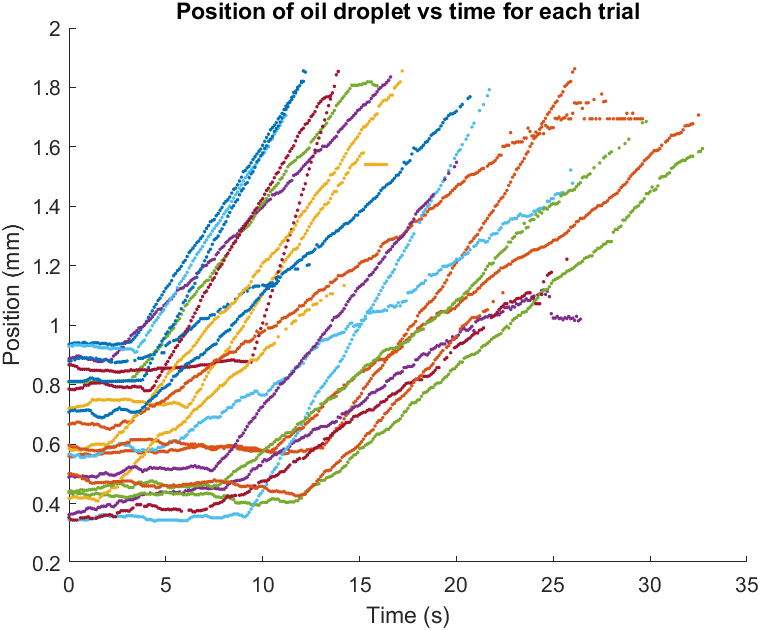
\includegraphics[width=0.45\textwidth]{figures/trialsPositionData.png}
  %\caption{Recorded position vs time data for different trials.}
  %\label{trialsPositionData}
%\end{figure}


\subsubsection{Goodness of Fit Analysis}


% A pretty good guide to formatting figures can be found at \url{https://en.wikibooks.org/wiki/LaTeX/Floats,_Figures_and_Captions#Figures}.
% \\


\section{Discussion}

\subsection{What physical quantity is the same for the single slit and double slit?}
\subsection{Comparing the distance between the single-slit central maximum and first minimum and the double-slit central maximum and first diffraction minimum}
\subsection{What physical quantity determines where the amplitude of the interference peaks goes to zero?}
\subsection{Number of interference maxima in the central evelope for a double slit with blah}
Includes 4 and 5


\section{Conclusions}



\section{Appendix}
\subsection{MATLAB code} \label{matlabCodeAppendix}
The MATLAB code written for curve fitting can be found here: \url{https://drive.google.com/file/d/1c0KO0R8WdM1CrL4F9txuAp1ntuowPlMq/view?usp=sharing}.

\subsection{Python code} \label{pythonCodeAppendix}
The Python script for finding the greatest common divisor can be found here: \url{https://drive.google.com/file/d/10CvMsZ6msjA-Matb5f5PmR-HgmCZE7pj/view?usp=sharing}. The code is largely based on template code found here: \url{https://www.geeksforgeeks.org/gcd-in-python/}.

\subsection{Calculated values from trials}\label{resultsAppendix}
Results from all trials can be found in this Google Sheet: \url{https://docs.google.com/spreadsheets/d/1sMJJarb4c3VgZ53b7jxh8RtN70SFS16z6iwI3uXQok8/edit?usp=sharing}

\section{References}
%\printbibliography
\end{document}
